In this chapter,
we investigate the nature of \emph{semi-structured data}
on web pages,
as well as the techniques for handling them in
a question answering system.
As explained in Section~\ref{sec:rw-semi-structured-data},
a semi-structured knowledge source contains some form of structures,
but the schemata of such structures are not defined in advance.
For instance,
Figure~\ref{fig:openweb-running-ex} shows a web page
where hiking trails and their descriptions
are listed using a uniform structure.
However, there is no universal way
for presenting a list of hiking trails.
The webmaster gets to choose the pieces of information
to be presented in each entry
and how they should be laid out on the web page.
As such,
a different website might use a different data schema,
presenting different pieces of information in a different format.

\begin{figure}[t]
\centering
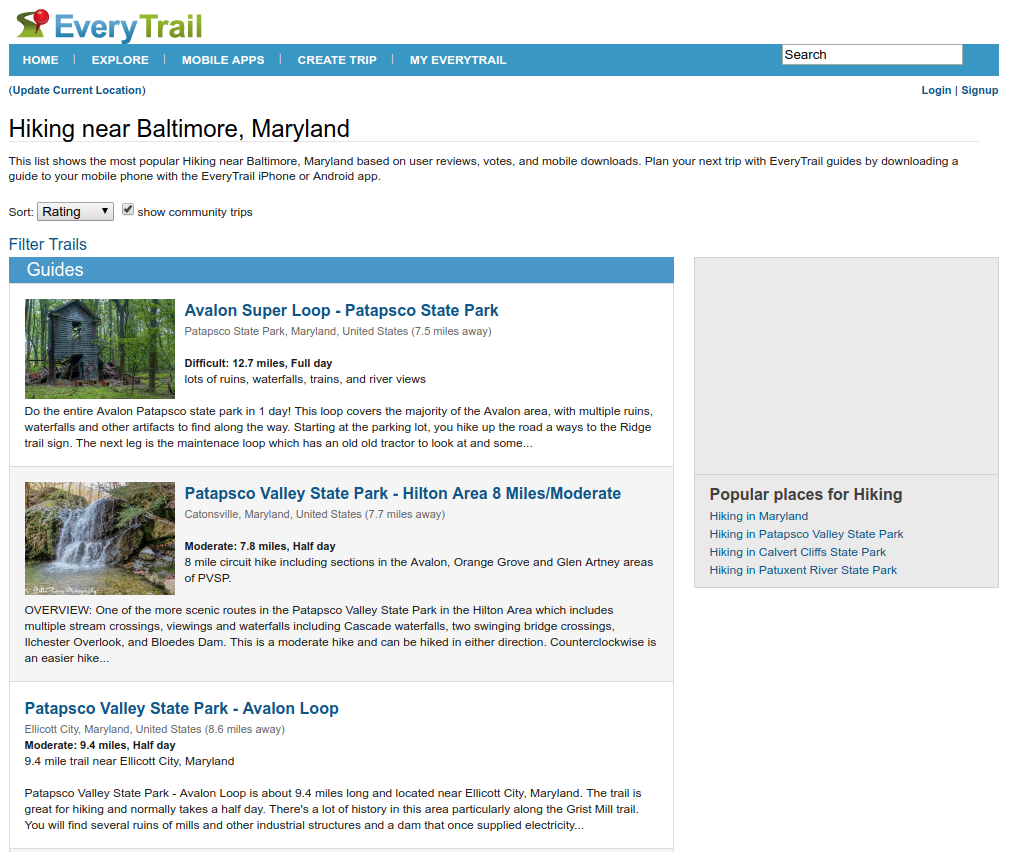
\includegraphics[scale=0.35]{figures/openweb/hiking-trails.png}
\caption[The list of hiking trails are presented in a semi-structured format on a web page.]{
The list of hiking trails are presented in a semi-structured format
on a web page. We consider the task of extracting
the specified list of entities
(e.g., \nl{hiking trails near Baltimore})
from the web page.}
\label{fig:openweb-running-ex}
\end{figure}

% Then in Section~\ref{sec:openweb},
% we consider the task of
% extracting a specified list of entities
% from the semi-structured data on the web page.
% (e.g., \nl{list of president names} $\to$
% \{``George Washington'', ``John Adams'', \dots\}).
% This task increases the focus on the structured part of the
% web page: the entity strings are to be extracted
% from the HTML elements with a coherent structure
% (e.g., cells from the same column of a table,
% or the header of each page section).

% Section~\ref{sec:openweb-compositional}
% gives several examples from
% our tasks that require compositional reasoning,
% which will serve as a motivation for the more complex task
% in later chapters.
% Finally, Section~\ref{sec:webpage-discussion}
% discusses related works on automated web interaction
% and information extraction from web documents.

To aid our investigation,
we consider the task of
extracting a specified list of entities
from the semi-structured data on the web page.
Concretely, given a natural language query
describing an entity category
and a relevant web page,
the task is to extract entities
that belong to the category from the page.
For example,
from the web page in Figure~\ref{fig:openweb-running-ex}
the question \nl{(What are) hiking trails near Baltimore}
should be mapped to the the list
\{\nl{Avalon Super Loop}, \nl{Patapsco Valley State Park}, \dots\}.
% Unlike information extraction from unstructured text
% \cite{hearst1992automatic,mintz2009distant,fader2014open},
% we can leverage the structured information on the web page:
% HTML elements containing entities of the same category
% usually have coherent structural properties.
% For instance, a web page showing a top-10 list
% usually have the ten entities as headers of the same level,
% and a web page with an information table might have
% the entities inside a single column of the table
% (excluding the column header).
We particularly focus on the semi-structured part of the
web page: the entity strings are expected to be extracted
from the HTML elements with a coherent structure
(e.g., cells from the same column of a table,
or the header of each page section).

We first formalize the task and give a few examples
from the \Sc{OpenWeb} dataset we collected for the task.
Afterward, we introduce \emph{extraction path},
an XPath-like latent selector
that selects HTML elements
that share the same structure.
The selected elements are then scores using
features that capture the homogeneity
of structural and linguistic information in the elements.
Finally, we present the experimental results of models
that were trained to generate good extraction paths.

\paragraph{Reference.}
The results described in this section have been published as
\citet{pasupat2014extraction}.

\section{The entity list extraction task}

\paragraph{Task.}
Given a web page $w$ (e.g., Figure~\ref{fig:openweb-running-ex})
and a natural language query $x$
(e.g., \nl{hiking trails near Baltimore}),
the task is to extracts a list $y$ of entities
that satisfy the query $x$
from the web page
(e.g., $y=$
\{\nl{Avalon Super Loop}, \nl{Patapsco Valley State Park}, \dots\}).

\paragraph{Dataset.}
We collected a new dataset, \Sc{OpenWeb},
with a diverse set of queries and web pages.
The data collection process is as follows:

\begin{enumerate}
\item
We used the method from \citet{berant2013freebase}
to generate a diverse set of search queries.
Specifically, we used the Google Suggest API,
which takes a partial query
(e.g., \nl{list of \blank movies})
and outputs complete queries
(e.g., \nl{list of horror movies}).

The queries were generated using breadth-first search
over the query space.
We started with the seed partial queries
\nl{list of $\bullet$\blank}
where $\bullet$ is one or two initial letters
(e.g., \nl{list of pr\blank}).
In each iteration, we called the Google Suggest API
to complete the queries,
and then applied the transformation rules in
Table~\ref{tab:openweb-suggest}
to generate more partial queries.
We ran the procedure until we obtained 100K queries.

\begin{table}[t]
\centering
\begin{tabular}{ll} \toprule
\textbf{Full query} & \textbf{New partial queries} \\
\midrule
list of $X$ IN $Y$
&list of $X$ \blank \\
where IN is a preposition
&list of \blank $X$ \\
(\emph{list of $[\text{hotels}]_X$ in $[\text{Guam}]_Y$})
&list of $X$ IN \blank \\
&list of \blank IN $Y$  \\
\midrule
list of $X$ CC $Y$
&list of $X$ \blank \\
where CC is a conjunction
&list of \blank $X$ \\
(\emph{list of $[\text{food}]_X$ and $[\text{drink}]_Y$})
&list of $Y$ \blank \\
&list of \blank $Y$ \\
\midrule
list of $X$ $w$
&list of $w$ \blank \\
(\emph{list of $[\text{good 2012}]_X$ $[\text{movies}]_w$})
&list of \blank $w$ \\
&list of $X$ \blank  \\
\bottomrule
\end{tabular}
\caption[
Rules for generating new partial queries
from complete queries.
]{Rules for generating new partial queries
from complete queries.
($X$ and $Y$ are sequences of words; $w$ is a single word.)}
\label{tab:openweb-suggest}
\end{table}

\item
For each query,
we downloaded the top 2--3 Google search results,
sanitized the web pages,
and randomly submitted 8000 web pages
along with their associated queries
to Amazon Mechanical Turk.
Each worker must either mark the web page
as irrelevant or identify the first, second,
and last entities (as strings) according to the query.
The dataset only contains examples where at least
two workers agreed on the three entities.
\end{enumerate}

The first, second, and last entities of the list
are used as a surrogate for the full list,
which is tedious to annotate.
We say that a list $y$ is \emph{consistent}
with the annotation if its first, second, and last entries
match the annotation.

\paragraph{Statistics.}
The \Sc{OpenWeb} dataset contains
2,773 examples from 2,269 distinct queries.
The queries span a variety of topics
from the more common ones
(e.g., movies, companies, characters)
to more obscure ones
(e.g., enzymes, proverbs, headgears).
The web pages are also diverse:
they come from 1,438 different web domains,
of which 83\% appears only once in the dataset.

Figure~\ref{fig:openweb-dataset} shows 
several queries and web pages from the dataset.
Besides the wide range of queries,
another main challenge of the dataset comes from
the diverse data representation formats such as 
tables, grids, lists, headings, and paragraphs.

\begin{figure}[t]
\centering
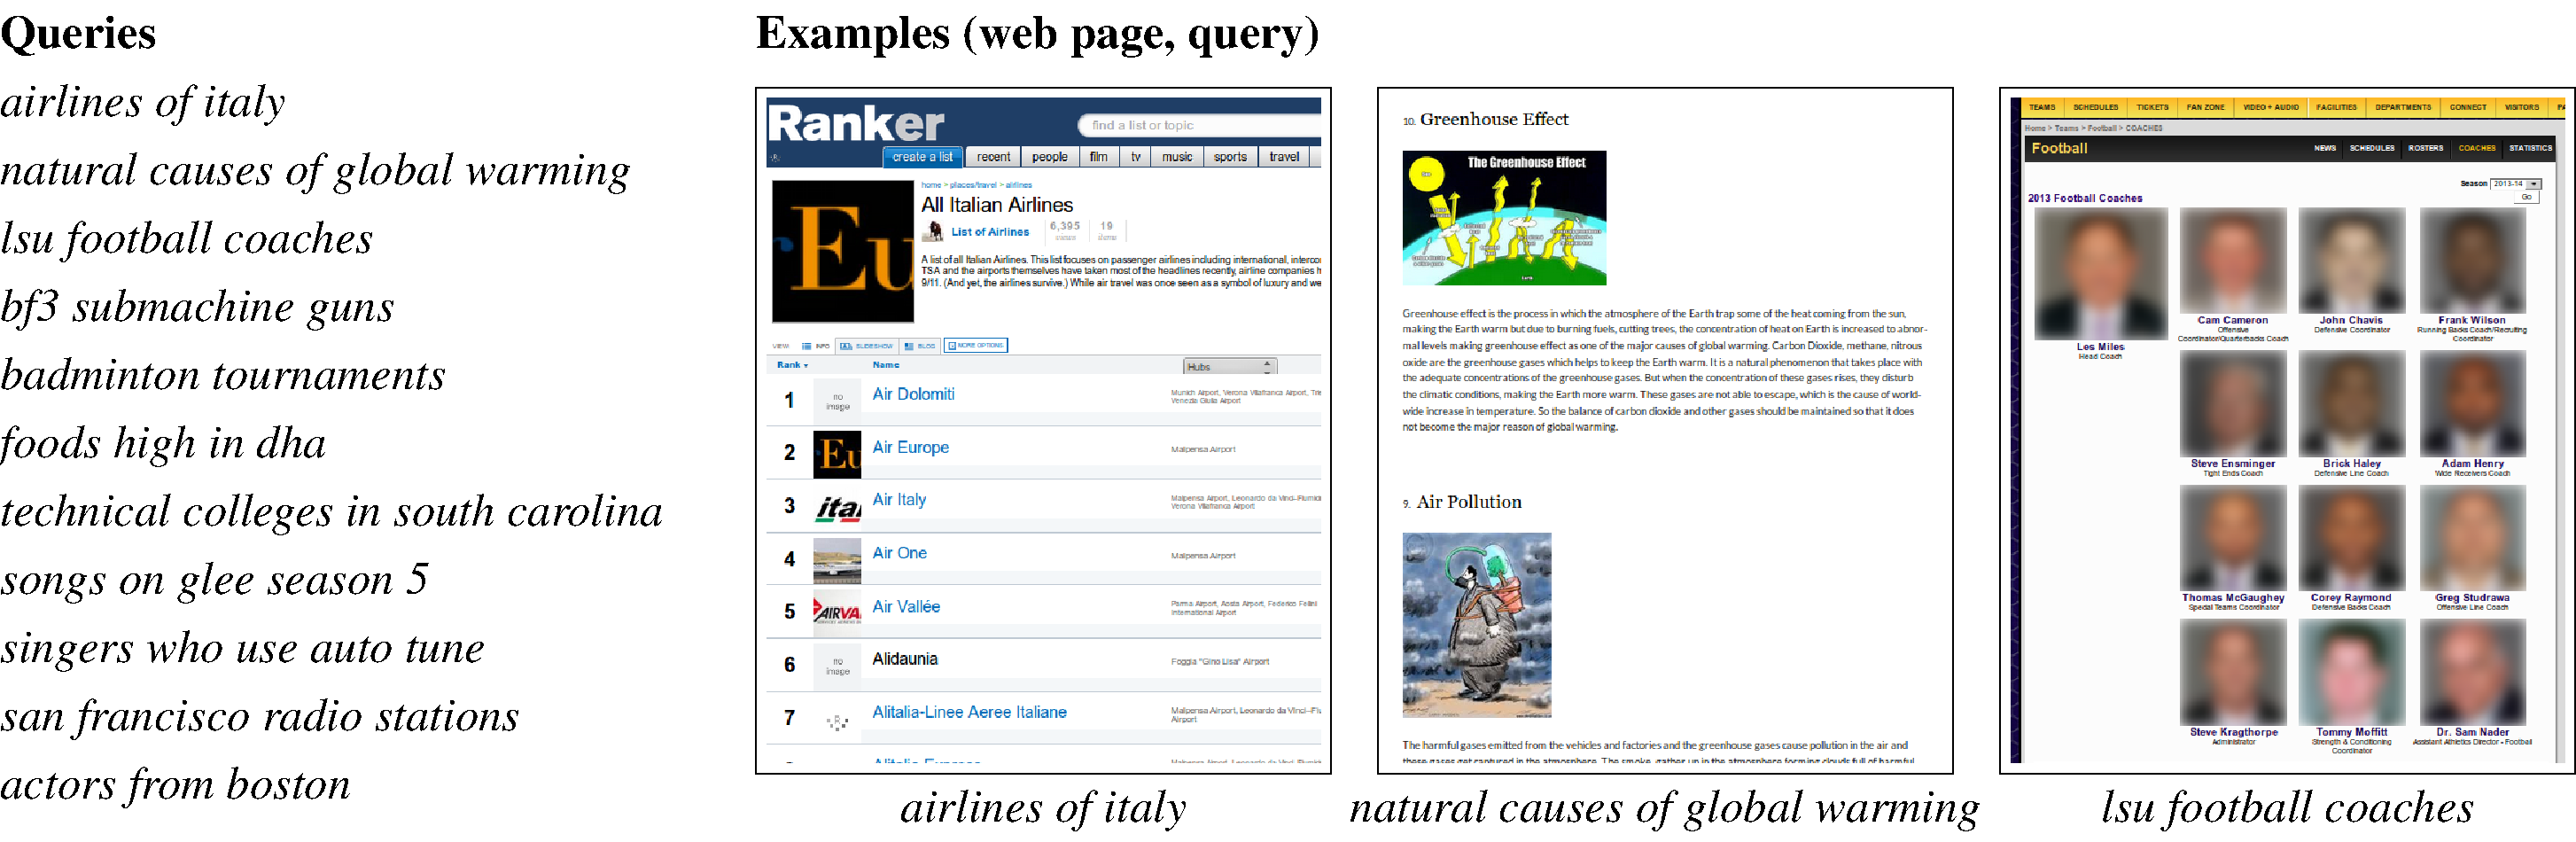
\includegraphics[width=\textwidth]{sfig/openweb.slides/extractionDataset.pdf}
\caption{Some examples illustrating the diversity of queries and web pages from the \Sc{OpenWeb} dataset.}
\label{fig:openweb-dataset}
\end{figure}


\section{Representation of the web page}\label{sec:openweb-representation}
The set of web pages across web domains form
a semi-structured knowledge source:
different web pages encode similar information
with different data schemata.
This schema mismatch sometimes manifests
even within the same web domain.
For example, while Wikipedia has guidelines on how
certain categories of articles should be formatted,
the data schemata still diverge drastically
between articles.

To handle arbitrary data schemata,
we propose to use a generic domain-independent structure
to represent web pages.
In particular,
we use the Document Object Model (DOM)
to represent the given web page $w$
as a tree of objects.
Unlike the full HTML DOM standard which includes multiple types of nodes
(e.g., text nodes and comment nodes),
we use a simplified representation
where all tree node are element nodes,
as shown in Figure~\ref{fig:openweb-extraction-path}.
For each DOM tree node,
we consider its HTML properties
(tag name and HTML attributes)
as well as its text content.
(The text content of non-leaf nodes
is the concatenation of all text content
within the subtree.)


\section{Extraction paths}\label{sec:extraction-paths}

We use latent \emph{extraction paths} $z$
to model the process of extracting entities
from the semi-structured web page $w$.
An extraction path is a simplified XML path (XPath) such as
\begin{equation}
z = \T{/html/body/table[2]/tr/td[1]}
\label{eqn:ex-xpath}
\end{equation}

Formally, an extraction path is a sequence of
\emph{path entries},
where each path entry is either a tag name (e.g., \T{tr})
or a tag name with an index (e.g., \T{td[1]}).
An extraction path $z$ can be executed on
the web page $w$ to get
$\deno{z}{w}$,
a list of matching HTML elements,
as follows:
\begin{itemize}
\item 
The base extraction path $z =$ \T{/html}
executes to a list containing
only the root \T{<html>} element of $w$.
\item
To execute $z\T{/}t$
(where $z$ is an extraction path and $t$ is a tag):
for each element $e \in \deno{z}{w}$,
select all children with tag $t$ of $e$.
Compile the selected elements into a list.
\item
To execute $z\T{/}t[i]$
(where $z$ is an extraction path, $t$ is a tag, and $i$ is an index):
for each element $e \in \deno{z}{w}$,
consider all children with tag $t$ of $e$,
and then select the $i$th one (1-indexed)
if there are at least $i$ such children.
Compile the selected elements into a list.
\end{itemize}

For example, as illustrated in
Figure~\ref{fig:openweb-extraction-path},
the extraction path
$z = \T{/html/body/table[2]/tr/td[1]}$
executes to the
first cell in each row of the second table on the page.
Note that all lists of elements are sorted
by the order they appear in the pre-order traversal
of the DOM tree.

\begin{figure}
\centering
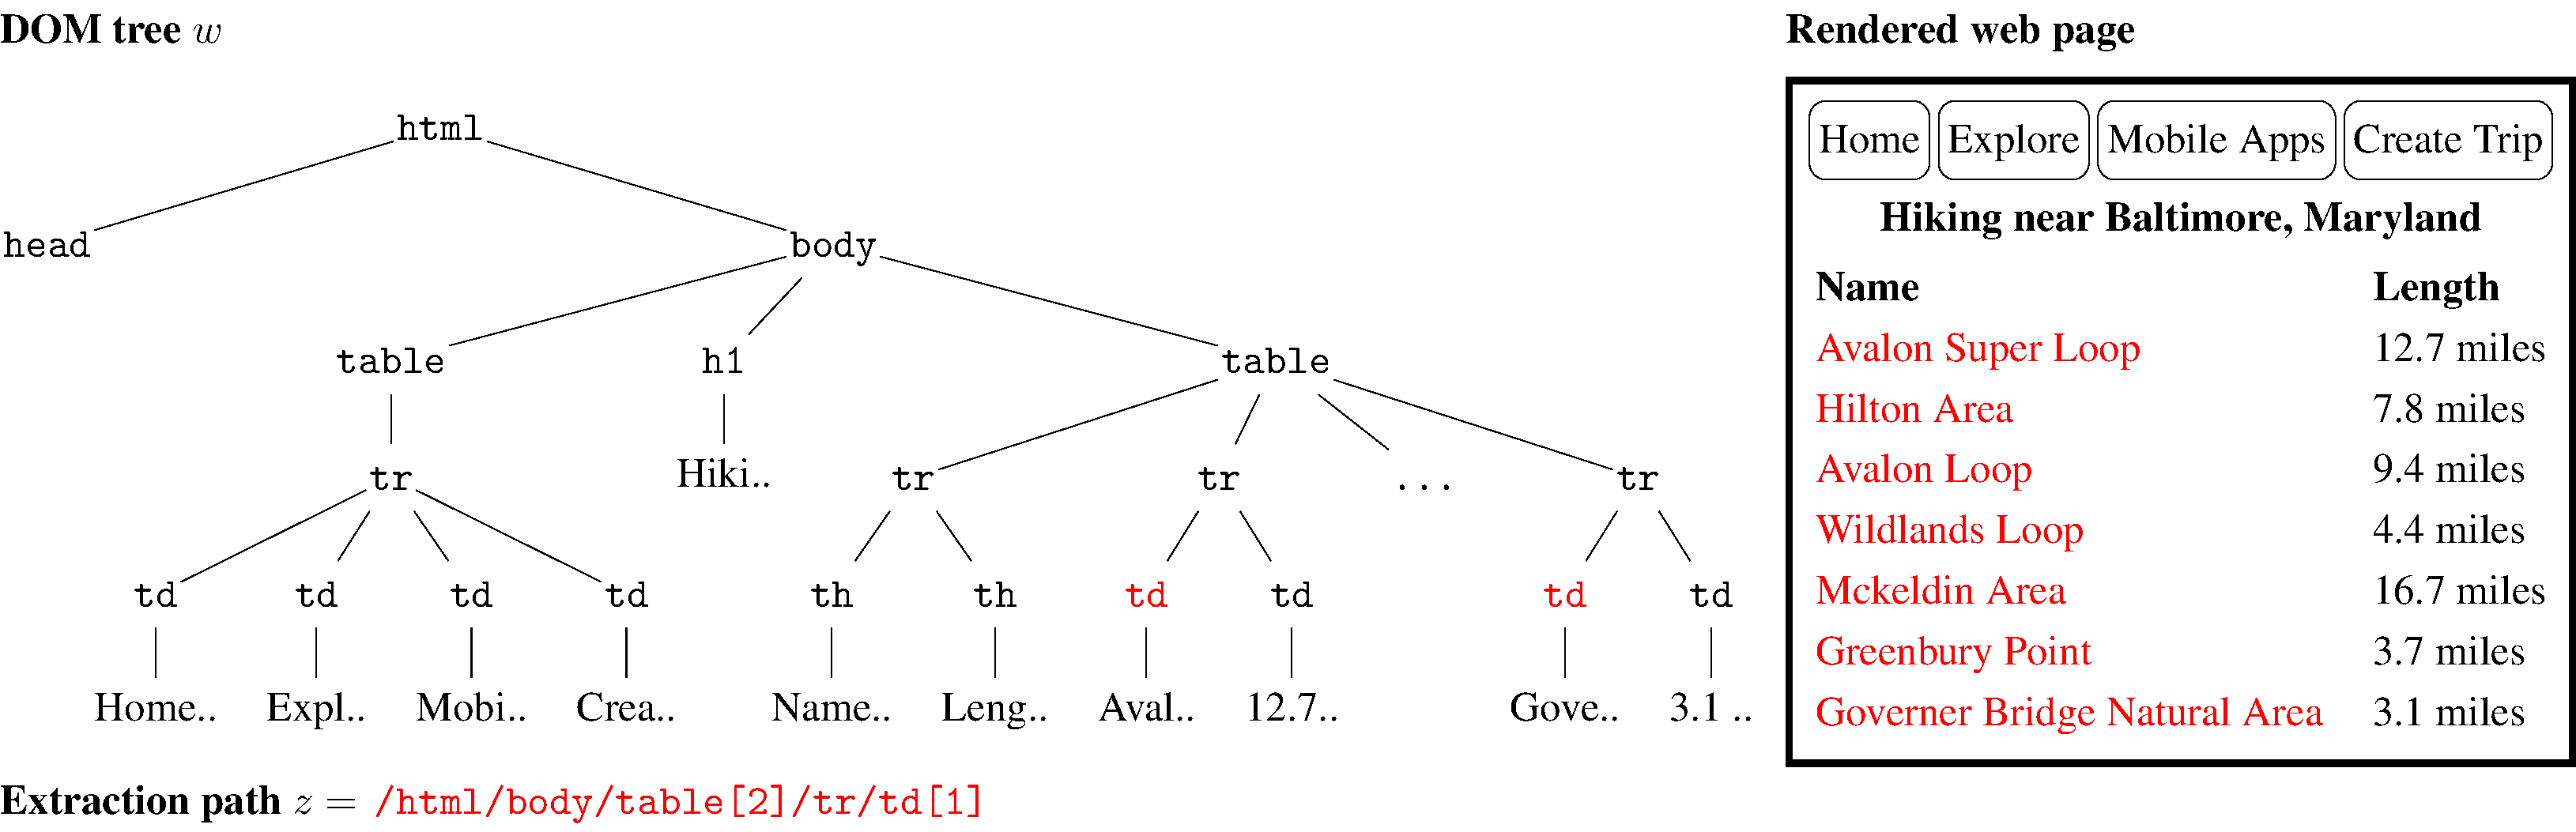
\includegraphics[width=\textwidth]{sfig/openweb.slides/extractionExample.pdf}
\caption[
Example of a DOM tree an extraction path.
]{A simplified example of a DOM tree of the web page $w$
and an extraction path $z$,
which selects a list of entity strings
$y = \deno{z}{w}$ from the web page (highlighted in {\color{red}red}).}
\label{fig:openweb-extraction-path}
\end{figure}

From the list $\deno{z}{w}$ of elements,
we can extract a list $y$ of entity strings
by compiling the text contents
of all elements in $\deno{z}{w}$
that are shorter than 140 characters.
This filtering is employed to control the search space.
This means an extraction path might yield an empty list of entities
(e.g., \T{/html/body/div[1]/p} gives no entities
if all the selected \T{<p>} elements contain
more than 140 characters).

\paragraph{Generating extraction paths.}
From a given web page $w$,
we can generate a set $\Mc{Z}(w)$ of candidate extraction paths
as follows.
For each element in the DOM tree,
we find an extraction path that selects only that element
(using only the indexed path entries),
and then generalizes the path by removing
any subset of indices of the last $k$ path entries.
For instance, when $k = 2$,
an extraction path ending in
\dots\T{/tr[5]/td[2]}
will be generalized to
\dots\T{/tr[5]/td[2]},
\dots\T{/tr/td[2]},
\dots\T{/tr[5]/td}, and
\dots\T{/tr/td}.
This generalization step allows us to select
multiple elements of the same structure
(e.g., table cells from the same column,
or list items from the same section).
We keep any generalized extraction path
where the extracted list of entities contain at least two entities.
Note that several extraction paths
might produce the same list of entities.

We use $k = 8$ in our experiments,
which gives at most $2^8$ generalized extraction paths
for each element.
Among the development examples of the \Sc{OpenWeb} dataset,
we generate on average approximately 8500 extraction paths,
which evaluate to approximately 1200 unique entity lists.

\section{Approach}
Given a query $x$ and a web page $w$,
we generate a set $\Mc{Z}(w)$
of candidate extraction paths $z$ as described
in Section~\ref{sec:extraction-paths}.
We then choose $z \in \Mc{Z}$ with the highest
model probability
$p_\theta(z \mid x, w)$
and extract the list of entities from $z$.

\paragraph{Model.}
From the query $x$ and the web page $w$,
we define a log-linear distribution over
the extraction paths in $\Mc{Z}(w)$ as
\begin{equation}
p_\theta(z \mid x, w) \propto \exp\crab{\theta^\top \phi(x,w,z)},
\end{equation}
where $\theta$ is the parameter vector
and $\phi(x,w,z)$ is the feature vector.

We train the model by maximizing the log-likelihood
of the extraction paths that
produce entity lists consistent with the annotation
(first, second, and last entities).
From training examples $(x\i, w\i, c\i)$,
where the indicator function $c\i(z)$ is 1 if
$z$ is consistent with the annotation and 0 otherwise,
we seek $\theta$ that maximizes
\begin{equation}
J(\theta) := 
\sum_{i} \log p_\theta(c\i = 1 \mid x\i, w\i) - \Omega(\theta)
\end{equation}
where
\begin{equation}
p_\theta(c = 1 \mid x, w)
= \sum_{z \in \Mc{Z}(w)} p_\theta(z \mid x, w)\,c(z)
\end{equation}
and $\Omega(z) = \frac{\lambda}{2}\norm{\theta}_2^2$
(with $\lambda = 0.01$)
is a regularization term.
We optimize $\theta$ with AdaGrad \cite{duchi10adagrad},
running for 5 epochs over the training data.

\section{Feature extraction}\label{sec:openweb-features}

The selected HTML elements from the web page $w$
contains both structured information
(e.g., their locations in the DOM tree)
and unstructured information
(e.g., their text contents).
As such,
we define the feature vector $\phi(x, w, z)$
as a concatenation of two types of features:
\emph{structural features} $\phi_\Mr{s}(w,z)$
which capture structured information of the HTML elements,
and \emph{denotation features} $\phi_\Mr{d}(x, y)$
which capture the linguistic information
of the extracted entity list $y$.

\begin{figure}
\centering
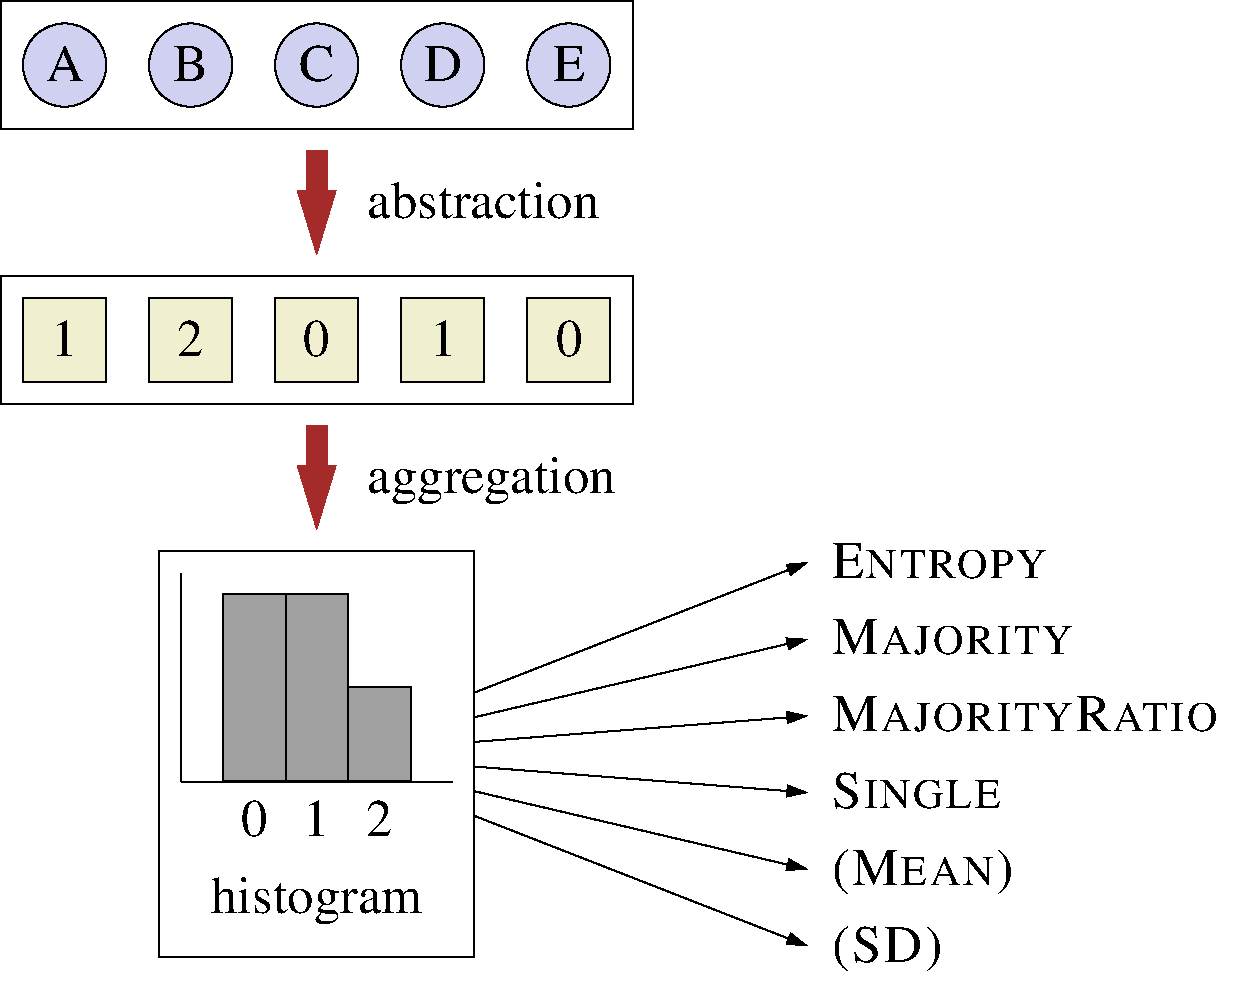
\includegraphics[width=0.5\textwidth]{sfig/openweb.slides/extractionFeatureRecipe.pdf}
\caption[
The recipe for defining features on a list of objects.
]{
The recipe for defining features on a list of objects:
(i) the \emph{abstraction} step converts list elements into abstract values;
(ii) the \emph{aggregation} step defines features using the histogram of the abstract values.}
\label{fig:openweb-recipe}
\end{figure}

\paragraph{Recipe for defining features on lists.}
Many of our features are defined on a list of objects
(e.g., a list of HTML elements or a list of entity strings).
When defining such features,
we want to incorporate the information about
individual list members,
as well as how the list looks like as a whole
(e.g., whether the members are diverse in some property).
As illustrated in Figure~\ref{fig:openweb-recipe},
we propose the following two-step recipe for generating
features from a list:

\begin{enumerate}
\item
\textbf{Abstraction.}
We map each list member to an abstract value
by extracting one of its properties.
For instance, we can map each each HTML element
to its number of children,
or map each entity string to its part-of-speech tag sequence.
\item
\textbf{Aggregation.}
We create a histogram of the abstract values,
and then define features based on the following statistics
of the histogram:
\begin{itemize}
\item \Sc{Entropy}: entropy normalized to the maximum value of 1.
The \Sc{Entropy} is 0 if all abstract values are identical,
and is 1 if all abstract values are distinct.
\item \Sc{Majority}: the most frequent abstract value.
\item \Sc{MajorityRatio}: percentage of abstract values
sharing the \Sc{Majority} value.
\item \Sc{Single}: whether all abstract values are identical.
\end{itemize}
For abstract values with finitely many possible values
(e.g., part-of-speech tags),
we also use the normalized count of each value as a feature.
And for numeric abstract values,
we also use the mean (\Sc{Mean}) and standard deviation (\Sc{SD}).
In our implementation,
real-valued features are converted to indicator features by binning.
\end{enumerate}

We use the recipe above to define structural features
and denotation features.
Figure~\ref{fig:openweb-features}
demonstrates some features we can extract from
the example in Figure~\ref{fig:openweb-extraction-path}.

\begin{figure}[t]
\centering
\begin{tabular}{cc}
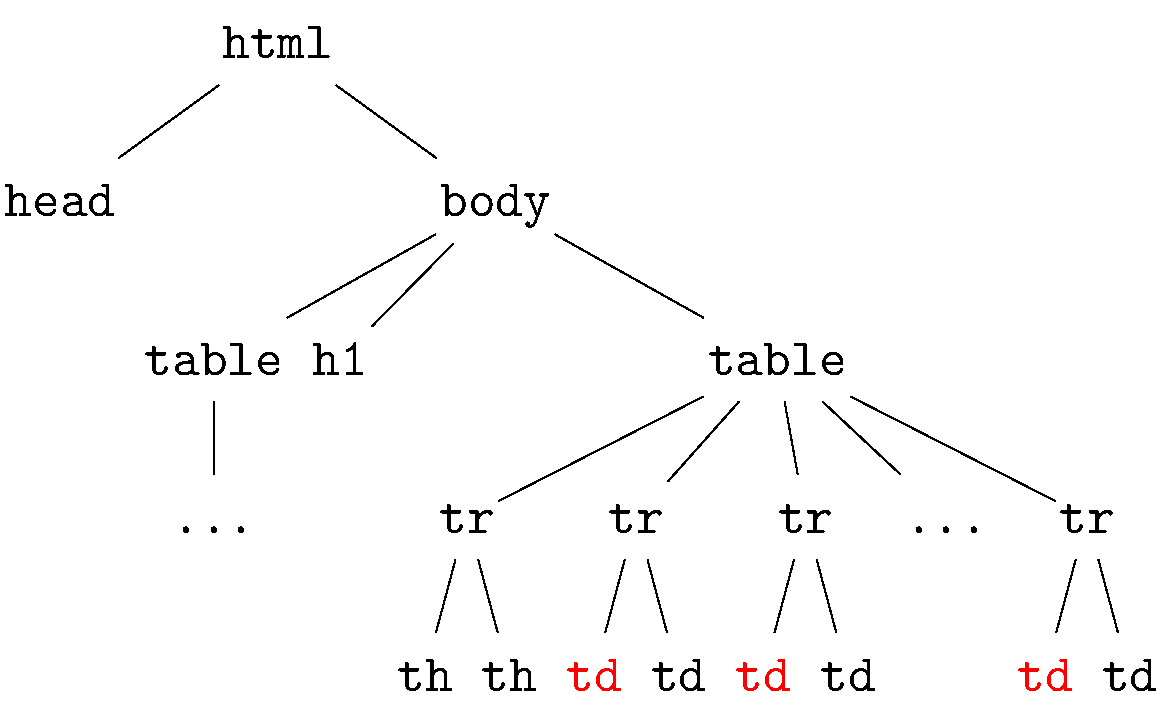
\includegraphics[scale=0.35]{sfig/openweb.slides/extractionFeatureStructural} &
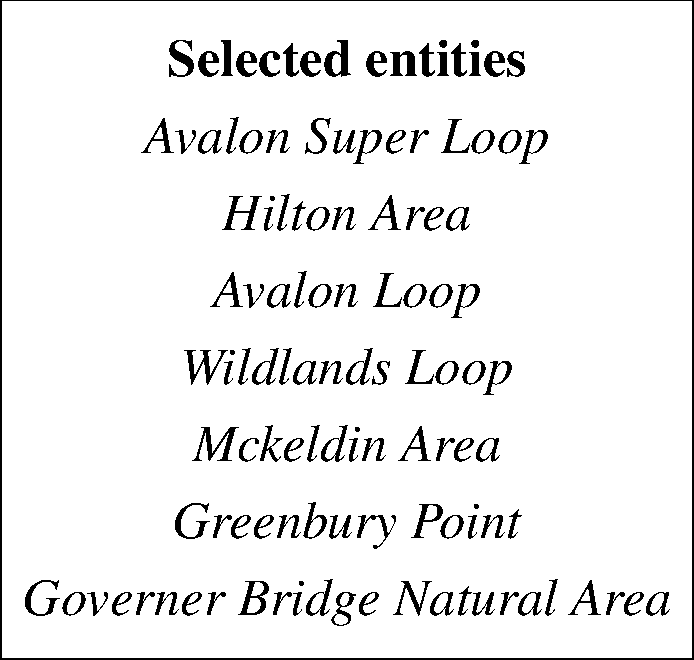
\includegraphics[scale=0.35]{sfig/openweb.slides/extractionFeatureDenotation} \\
\begin{tabular}[t]{ll} \toprule
\textbf{Structural feature} & \textbf{Value} \\ \midrule 
Features on selected nodes: \\
\quad\textsc{Tag-Majority} = \texttt{td} & 1\\
\quad\textsc{Index-Entropy} & 0.0 \\
Features on parent nodes: \\
\quad\textsc{ChildrenCount-Majority} = 2 & 1 \\
\quad\textsc{Parent-Single} & 1\\
\quad\textsc{Index-Entropy} & 1.0 \\
\quad\textsc{HeadHole} {\small (The first node is skipped)} & 1\\
Features on grandparent nodes: \\
\quad\textsc{PageCoverage} & 0.6 \\
\ldots & \ldots \\
\bottomrule
\end{tabular} &
\begin{tabular}[t]{ll} \toprule
\textbf{Denotation feature} & \textbf{Value} \\ \midrule 
\textsc{WordsCount-Mean} & 2.42 \\
\textsc{PhraseShape-Majority} = \texttt{Aa Aa} & 1 \\
\textsc{PhraseShape-MajorityRatio} & 0.71 \\
\textsc{WordShape-Majority} = \texttt{Aa} & 1 \\
\textsc{PhrasePOS-Majority} = NNP NN & 1\\
\textsc{LastWord-Entropy} & 0.74 \\ 
\textsc{WordPOS} = NN {\small (normalized count)} & 0.53 \\
\ldots & \ldots \\
\bottomrule
\end{tabular}
\end{tabular}

\caption[
A small subset of features from the example \emph{hiking trails near Baltimore}.
]{A small subset of features from the example \emph{hiking trails near Baltimore} in Figure~\ref{fig:openweb-extraction-path}.}
\label{fig:openweb-features}
\end{figure}

\paragraph{Structural features.}
Although different web pages represent data in different formats,
they still share some common hierarchical structures in the DOM tree.
We use structural features $\phi_\Mr{s}(w, z)$
to capture the structural information
from the extraction path $z$ and the selected elements $\deno{z}{w}$:

\begin{itemize}
\item \textbf{Features on the list of selected elements.}
We apply our recipe on the list of elements in $\deno{z}{w}$ using
the following abstract values of each element:
\begin{itemize}
\item The HTML \Sc{Tag} and attributes (\Sc{Id}, \Sc{Class}, \Sc{Href}, etc.)
\item \Sc{ChildrenCount}: the number of children of the element in the DOM tree.
\item \Sc{SiblingCount}: the number of siblings in the DOM tree.
\item \Sc{Index}: the position among its siblings.
\item \Sc{Parent}: the parent element
(e.g., the resulting \Sc{Parent-Single} feature indicates
that all elements share the same parent).
\end{itemize}

\item \textbf{Hole features.}
If the extraction path does not select all elements
in the same DOM tree level,
it is likely that the selection is incorrect.
For instance, an extraction path ending in \dots\T{/ul[1]/li/a}
selects links inside an unlabeled list.
However, if some list entries do not have links for some reason,
then the selected list will be incomplete.
In this case, it is preferred to use \dots\T{/ul[1]/li}
to select the list entries themselves instead.

To capture this intuition,
we define a \Sc{NoHole} feature
if all parents of the selected elements
has at least one of the selected elements as a child.
For the example above,
if some list entries \dots\T{/ul[1]/li} do not have links,
then the extraction path \dots\T{/ul[1]/li/a}
will not generate a \Sc{NoHole} feature.
To account for the common case of selecting table cells (\dots\T{/tr/td[$i$]}),
where the first row \T{<tr>} usually contains \T{<th>} instead of \T{<td>},
we define a \Sc{HeadHole} feature
if only the first parent is violating our criterion.

\item \textbf{Coverage feature.}
We define a real-valued feature \Sc{PageCoverage}
as the number of HTML elements that are descendents 
of the selected elements, divided by the total number of elements
on the web page.

\item \textbf{Features on ancestor elements.}
We also define the same feature set on the list of ancestors
of the selected elements.
In our experiments, we traverse up to 5 levels of ancestors
and define separate structural features on each level.

\end{itemize}

\paragraph{Denotation features.}
Structural features are not powerful enough
to distinguish entity lists with the same structure
(e.g., different columns of the table,
or different lists on the same web page).
To resolve this issue,
we define denotation features $\phi_\Mr{d}(x, y)$
on the entity list $y$ extracted from the selected elements:

\begin{itemize}
\item \textbf{Linguistic features.}
We observe that the correct entities often share 
some linguistic features.
For example, people and place names usually contain
2--3 word tokens with part-of-speech tag NNP (proper noun).
In contrast, incorrect lists of elements
(e.g., various \T{<div>} elements across the page)
tend to have texts of diverse lengths and linguistic tags.
With this reasoning, we apply our recipe on the list
of entity strings using the following abstract values
of each string:
\begin{itemize}
\item \Sc{WordCount}: number of tokens.
\item \Sc{PhraseShape}: abstract shape of the string
(e.g., \nl{Stanford University} becomes ``\T{Aa Aa}'').
\item \Sc{WordShape}: abstract shape of each word.
The features are defined on the list of words instead of the
list of entity strings.
\item \Sc{FirstWord} and \Sc{LastWord}
\item \Sc{PhrasePOS}: the part-of-speech sequence
of the whole string.
\item \Sc{WordPOS}: part-of-speech of each word.
Like \Sc{WordShape},
the features are defined on the list of words instead.
\end{itemize}

\item \textbf{Query-denotation features.}
Different query types denote entities
with different linguistic properties.
For instance, queries \nl{mayors of Chicago}
and \nl{universities in Chicago}
will produce entities of different lengths,
path-of-speech sequences, and word distributions.
This suggests incorporating features that depend
on the query $x$.

To this end, we define features of the form
$(f(y), g(x))$, where $f(y)$ is a linguistic feature
as described above, and $g(x)$ is the category of the query $x$.
For our experiments, we manually classify
the queries into 7 categories:
person, media title, location/organization,
abstract entity, word/phrase, object name, and miscellaneous.
In an actual system, the queries
should be classified automatically instead,
but we leave this as future work.
\end{itemize}

As the query-denotation features require
additional manual annotation,
we exclude them from the main experiments.
Instead,
we will investigate the effect of query-denotation features
in our model analysis (Section~\ref{sec:openweb-analysis}).

\section{Experiments}

We evaluate our model on the \Sc{OpenWeb} dataset.
The main evaluation metric is \emph{accuracy}:
the fraction of examples where
the model predicts an entity list consistent with the annotation.
We also report \emph{accuracy at 5},
the fraction of examples where one of the
five highest-scoring extraction path
yields a consistent entity list.
Finally, we report the \emph{oracle} score,
the fraction of examples where the model can
find at least one consistent entity list
among all extraction paths.

To measure how the consistency-based accuracy
tracks the actual correctness,
we sampled 100 web pages which have at least
one valid extraction path and manually annotate
them with the full entity lists.
We found that in 85\% of the examples,
the longest consistent list $y$ is the correct list,
and many lists in the remaining 15\%
miss the correct list by only a few entities.

\newcommand\sufpat[5]{\{\T{#1}, \T{#2}, \T{#3}, \T{#4}, \T{#5}\}}

\begin{table}[t]
\centering
\begin{tabular}{lr} \toprule
\textbf{Path suffix pattern} & \textbf{Count} \\ \midrule
\sufpat{a}{table}{tbody}{td[*]}{tr} & 1792 \\
\sufpat{a}{tbody}{td[*]}{text}{tr} & 1591 \\
\sufpat{a}{table[*]}{tbody}{td[*]}{tr} & 1325 \\
\sufpat{div}{table}{tbody}{td[*]}{tr} & 1259 \\
\sufpat{b}{div}{div}{div}{div[*]} & 1156 \\
\sufpat{div[*]}{table}{tbody}{td[*]}{tr} & 1059 \\
\sufpat{div}{table[*]}{tbody}{td[*]}{tr} & 844 \\
\sufpat{table}{tbody}{td[*]}{text}{tr} & 828 \\
\sufpat{div[*]}{table[*]}{tbody}{td[*]}{tr} & 793 \\
\sufpat{a}{table}{tbody}{td}{tr} & 743 \\ \bottomrule
\end{tabular}
\caption[
Top 10 path suffix patterns found by the baseline.
]{Top 10 path suffix patterns
found by the baseline.
We blank out the index numbers
and disregard the order of path entries,
making them a multiset instead of a sequence.
}\label{tab:openweb-baseline}
\end{table}

\paragraph{Baseline.}
As a baseline,
we list all 5-entry
suffixes of the correct extraction paths
in the training data,
and then sort the suffixes by frequency.
Table~\ref{tab:openweb-baseline}
shows the most frequent suffixes.
To increase generalization,
we blank out the index numbers
and discard the order of path entries.
At test time,
we choose an extraction path with the most
frequent suffix pattern.
The baseline should work reasonably well
if the web pages are relatively homogeneous.

\paragraph{Main results.}
We split the dataset into 70\% training and 30\% test data.
In addition to testing on test data,
we also report the results on 10 random 80-20 splits
of the training data.

\begin{table}[t]
\centering
\begin{tabular}{lcccc} \toprule
& \multicolumn{2}{c}{\bf 10 random splits} & \multicolumn{2}{c}{\bf Test data} \\
& \textbf{Acc} & \textbf{Acc@5} & \textbf{Acc} & \textbf{Acc@5} \\ \midrule
\textbf{Baseline} & 10.8 $\pm$ 1.3 & 25.6 $\pm$ 2.0 & 10.3 & 20.9 \\
\textbf{Our approach} & 41.1 $\pm$ 3.4 & 58.4 $\pm$ 2.7 & 40.5 & 55.8 \\
\textbf{Oracle} & 68.7 $\pm$ 2.4 & 68.7 $\pm$ 2.4 & 66.6 & 66.6 \\ \bottomrule
\end{tabular}
\caption[
Main results on the \Sc{OpenWeb} dataset.
]{Main results on the \Sc{OpenWeb} dataset
using the default set of features.
(Acc = accuracy, Acc@5 = accuracy at 5)}
\label{tab:openweb-main-results}
\end{table}

As reported in
Table~\ref{tab:openweb-main-results},
our approach gets a test accuracy of 40.5\%.
The oracle accuracy of 66.6\% reveals that there are
two categories of errors:
(i) \emph{coverage errors} (33.4\%),
which are when the system cannot find any
consistent entity list,
and (ii) \emph{ranking errors} (26.1\%),
which are when a consistent list of entities
exists but does not have the highest probability.

\begin{table}[p]\centering
\begin{tabular}{rp{5.5cm}p{6.5cm}r} \toprule
& \textbf{Reason} & \textbf{Example} & \textbf{Count} \\ \midrule
C1
& Answers and non-answer elements are selected by the same extraction path. 
& Select entries in the \nl{See Also} section
in addition to the content because they are all \texttt{<li>}.
& 48 \\ \midrule
C2
& HTML tag usage is inconsistent.
& The page uses both \texttt{<b>} and \texttt{<strong>} for headers
interchangeably.
& 16 \\ \midrule
C3
& The query applies to only some sections of the matching entities.
& Need to select only companies in China from the table of all Asian companies.
& 20 \\ \midrule
C4
& Answers are embedded in running text.
& Answers are in a comma-separated list.
& 13 \\ \midrule
C5
& Text normalization issues.
& Selected \nl{Silent Night Lyrics} instead of \nl{Silent Night}.
& 19 \\ \midrule
C6
& Other issues.
& Incorrect annotation / Entities are permuted when the web page is rendered
& 18 \\ \midrule
& \textbf{Total} & & 134 \\ \bottomrule
\end{tabular}

\caption{Breakdown of coverage errors from the development data.}\label{tab:webrep-coverage-errors}
\end{table}

\begin{table}[p]\centering
\begin{tabular}{rp{5.5cm}p{6.5cm}r} \toprule
& \textbf{Reason} & \textbf{Example} & \textbf{Count} \\ \midrule
R1
& Select non-content strings.
& Select navigation links, headers, footers, or sidebars.
& 25 \\ \midrule
R2
& Select entities from a wrong field.
& Select book authors instead of book names.
& 22 \\ \midrule
R3
& Select entities from wrong section(s).
& For the query \nl{schools in Texas},
select all schools on the page, or select the schools in Alabama instead.
& 19 \\ \midrule
R4
& Also select headers or footers.
& Select the table header in addition to the answers.
& 7 \\ \midrule
R5
& Select only entities with a particular formatting.
& From a list of answers, select only entities that are links (\T{<a>}).
& 4 \\ \midrule
R6
& Select headings instead of the contents or vice versa.
& Select the categories of rums in \T{<h2>} instead of the rum names in the tables.
& 2 \\ \midrule
R7
& Other issues.
& Incorrect annotation / Multiple sets of answers appear on the same page / etc.
& 9 \\ \midrule
& \textbf{Total} & & 88 \\ \bottomrule
\end{tabular}
\caption{Breakdown of ranking errors from the development data.}\label{tab:webrep-ranking-errors}
\end{table}

\section{Analysis}\label{sec:openweb-analysis}

Tables~\ref{tab:webrep-coverage-errors}~and~\ref{tab:webrep-ranking-errors}
show the breakdown of the coverage and ranking errors
on one of the development splits.

\paragraph{Analysis of coverage errors.}
From Table~\ref{tab:webrep-coverage-errors},
about 36\% of coverage errors happen when
the extraction path for the correct entities also 
captures irrelevant parts of the web page (Reason~C1).
For example, many Wikipedia articles contain
the \emph{See Also} section that lists
related articles in an unordered list
(\dots\T{/ul/li/a}).
This is problematic when the entities to be selected
are also represented in the same way.

Another main source of errors is the inconsistency
in HTML tag usage (Reason~C2).
For instance, some web pages use \T{<b>}
and \T{<strong>} interchangeably
for bold texts,
or switch between \T{<b><a>}\dots\T{</a></b>}
and \T{<a><b>}\dots\T{</b></a>} across entities.
Normalizing the web page,
using alternative web page representations,
or using a more expressive representation
than extraction paths could help reduce this type of errors.

\paragraph{Analysis of ranking errors.}
From Table~\ref{tab:webrep-ranking-errors},
a large number of errors are attributed to
selecting non-content elements such as
navigation links or content headings (Reason~R1).
It turns out that structural and linguistic
statistics of these elements can sometimes
be more coherent than those of the correct entities.
Since our features try to capture the
homogeneity of the selected elements,
the model can end up selecting these irrelevant elements.
A possible solution is to
detect the saliency of the element
and favor the elements that are in the content part
of the page.

\begin{table}[t]\centering
\begin{tabular}{lcc} \toprule
\textbf{Setting} & \textbf{Acc} & \textbf{Acc@5} \\ \midrule
All features & 41.1 $\pm$ 3.4 & 58.4 $\pm$ 2.7 \\
Oracle & 68.7 $\pm$ 2.4 & 68.7 $\pm$ 2.4 \\
\midrule
Structural features only & 36.2 $\pm$ 1.9 & 54.5 $\pm$ 2.5 \\
Denotation features only & 19.8 $\pm$ 2.5 & 41.7 $\pm$ 2.7 \\
\midrule
Query-denotation features only & 25.0 $\pm$ 2.3 & 48.0 $\pm$ 2.7 \\
Structural + query-denotation & 41.7 $\pm$ 2.5 & 58.1 $\pm$ 2.4 \\  \midrule
Concatenate a random web page + \\ \quad structural + denotation & 19.3 $\pm$ 2.6 & 41.2 $\pm$ 2.3 \\
Concatenate a random web page + \\ \quad structural + query-denotation & 29.2 $\pm$ 1.7 & 49.2 $\pm$ 2.2 \\
\bottomrule
\end{tabular}
\caption[
System accuracy with different feature and input settings on the development data.
]{System accuracy with different feature and input settings on the development data.
(Acc = accuracy, Acc@5 = accuracy at 5)}\label{tab:openweb-ablation}
\end{table}

\paragraph{Feature ablation.}
Table~\ref{tab:openweb-ablation}
shows the ablation results
on 10 development splits.
We observe while the structural features
are responsible for most of the accuracy,
denotation features is also helpful.
By examining the actual predictions,
we found that if there are multiple
parallel lists on the web page
(e.g., different columns of a tables),
denotation features help the system
select the correct list.
In contrast, structural features
act as a prior that
prevents the system from selecting
random entities outside the main part
of the web page.

\paragraph{Query-denotation features.}
The model so far does not include query-denotation features,
meaning that the input query $x$ is ignored entirely.
Despite this, since the web page
was obtained from a search engine,
the most prominent entities on the web pages
are likely to satisfy the query already,
and thus we were able to get some reasonable accuracy.

Table~\ref{tab:openweb-ablation}
shows that using only query-denotation features
(no structural features)
increases the accuracy over using 
normal denotation features
by 5.2\%.
When combined with structural features,
the query-denotation features help the model
select entities that are more appropriate for the query,
as shown in Table~\ref{tab:openweb-deno-example}.
However, it does not increase the
overall accuracy.
This is perhaps because the web page is already
related to the query as argued earlier.

\begin{table}[t]
\centering
\begin{tabular}{lll} \toprule
\textbf{Query} & \textbf{Default features} & \textbf{+ query-denotation} \\
\midrule
euclid’s elements book titles
& \nl{Prematter} & \nl{Book I. The fundamentals \dots} \\
(category = \emph{media title})
& \nl{Book 1} & \nl{Book II. Geometric algebra.} \\
& \nl{Book 2} & \nl{Book III. Theory of circles.} \\
& \dots & \dots \\ \midrule
soft drugs
& \nl{Hard drugs} & \nl{methamphetamine} \\
(category = \emph{object name})
& \nl{Soft drugs} & \nl{psilocybin} \\
& \nl{Some drugs cannot be classi\dots} & \nl{caffeine} \\
& \dots & \dots \\ \midrule
professional athletes
& ``\emph{Pistons-Knicks Game Becomes}
& \nl{Mike Richter} \\
with concussions
& \emph{\quad Site of Incredible Dance Battle}''
& \nl{Stu Grimson} \\
(category = \emph{person})
& \nl{Toronto Mayor Rob Ford \dots} & \nl{Geoff Courtnall} \\
& \dots & \dots \\ \bottomrule
\end{tabular}
\caption{The predictions after changing denotation features
into query-denotation features.}
\label{tab:openweb-deno-example}
\end{table}

To test query-denotation features
in scenarios where the most prominent elements
might not give correct entities,
we conduct experiments on a modified dataset
where in each example,
the original web page and an unrelated web page
are concatenated (in a random order).
We find that query-denotation features
(with structural features) significantly
improve the accuracy over using the normal
denotation features from 19.3\% to 29.2\%.


\section{Related work and discussion}
\label{sec:webpage-discussion}

\paragraph{Web page understanding.}
To understand the overall structure of web pages,
work on web page segmentation aims to segment the page
into semantically meaningful blocks
\cite{bing2014web,kreuzer2015quantitative},
identify salient parts of the web page
\cite{gamon2013identifying,shen2014webpage},
align the structures with the same semantics between web pages
\cite{kumar2011bricolage},
or detect the semantics of web page regions
\cite{spengler2010document,kumar2013webzeitgeist}.

\paragraph{Extracting information from web pages.}
Our presented approach is closely related to the work on
wrapper induction \cite{kushmerick1997wrapper}.
A wrapper is a function that takes the web page as input
and return the extracted information.
% For instance, our extraction path can be viewed as a wrapper.
Previous work on wrapper induction
mostly focuses on a small set of web domains,
and assume that the web pages follow a fixed template
\cite{muslea2001hierarchical,crescenzi2001roadrunner,cohen2002flexible,arasu2003extracting,dalvi2011automatic}.
Later work tries to generalize across web pages,
but relies on restricted data format \cite{wong2009scalable}
or prior knowledge of the web page structure
for the desired data to extract \cite{zhang2013automatic}.

Given a web page generated from a template
(e.g., a product listing page on an online shop),
previous work has also considered using
the regularity of web page elements
to extract structured information.
For instance, \citet{grigalis2014unsupervised}
extracts data records by looking at contiguous elements
that are visually similar,
and \citet{omari2016lossless}
factors the raw data from the web template.

Our setting differs from previous work on wrapper induction
in two major ways.
First, most previous works on wrapper induction
operate on a fixed website.
The induced wrapper only match the data schema of that website,
and is not likely to work on a different websites
or even a different version of the same website.
Similar to some previous work that generalize across pages
mentioned above
\cite{wong2009scalable,zhang2013automatic},
our approach does not make an assumption about the schema of the web page.
Second, in most wrapper induction systems,
the user specifies a few examples of entities to be extracted,
and the system tries to find wrappers that can extract
such entities.
Our setting has natural language as the specification
of what entities to extract,
which requires less effort from the user.
Note that 
while the query-dependent features has minor impact
on the overall extraction accuracy,
the features do help in scenarios where the most
prominent HTML elements on the page do not produce
the specified entities.

\paragraph{Collating information from web pages.}
Instead of extracting only the specified type of information,
one might want to mine and process all possible information
from a collection of web pages.
This can reveal corpus-level statistics that cannot be captured
by processing individual web pages.
For instance, WebTables \cite{cafarella2008webtables}
compiles a large corpus of web tables,
resulting in a corpus that can be used for many downstream tasks
such as deriving the correlation between data schemata (column headers).
Other works consider methods for processing
the mined data,
such as recovering the missing column headers \cite{venetis2011recovering}
or converting raw data to canonical formats
\cite{sarawagi2014open,embley2016converting}.

One way to view these families of information extraction methods
is to compare them with relation extraction from unstructured text (Section~\ref{sec:rw-ie}).
Wrapper induction and other query-based extraction methods
is parallel to relation extraction with
a predefined set of relations \cite{hearst1992automatic,mintz2009distant,miwa2016end}.
In contrast, WebTables and other works that collate information
from the structured parts of web pages
is parallel to open information extraction
\cite{banko2007open,fader11reverb,etzioni11openie,masaum2012open}.

\paragraph{Interacting with web pages.}
Previous work has considered a variety of interfaces
for humans to interact with web pages.
Some examples include
keystrokes \cite{spalteholz2008keysurf},
speech \cite{ashok2014wizard},
haptics \cite{yu2005haptics},
and eye gaze \cite{kumar2007eyepoint}.

In contrast to the methods above,
automated web scripts can be used for web page interaction
with minimal human intervention.
Most script frameworks refer to elements with logical selectors
such as CSS matchers and XPaths.
Due to the brittle nature of these selectors,
the script can break when the web page changes its layout,
or when the attributes of HTML elements are automatically generated
(either due to the web framework used or for obfuscation purposes)
\cite{hammoudi2016why}.

Previous work has proposed alternative methods
for referencing web elements in automated web scripts.
A few examples include Sikuli \cite{yeh2009sikuli},
which uses images of the elements,
and TagUI \cite{soh2017tagui},
which uses natural language.
These tools were designed for productivity,
but also have robustness as a side benefit.
For instance, even when an element changes its attributes
or location, a visual-based selector
will still be able to select it.

Instead of manually authoring the scripts,
previous work has also considered learning an agent
to perform actions on web page based on the given goal.
The agent can be learned
from demonstrations \cite{allen2007plow},
reinforcement learning
\cite{branavan08annotation,branavan09reinforcement}
or both \cite{shi2017wob,liu2018workflow}.

\paragraph{The need for compositionality.}

While doing error analysis,
we observe multiple examples that require
compositional understanding of the input query $x$
to obtain the correct answers.
A few of such examples are elaborated below:

%%%%%%%%%%

\begin{figure}[tp]
\centering
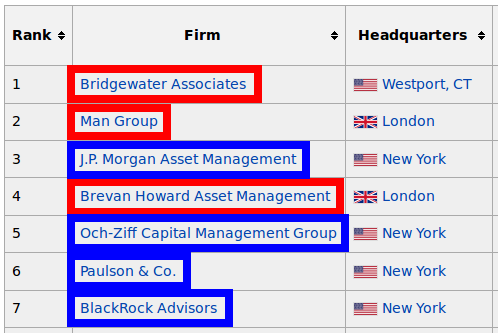
\includegraphics[scale=0.45]{figures/openweb/incorrect2-hedgefund.png}
\caption[
The query \nl{list of hedge funds in New York}
requires compositional understanding.
]{The query \nl{list of hedge funds in New York}
requires filtering the list of entities
by the value in the Headquarters column.}
\label{fig:openweb-hedgefund}
\end{figure}

\begin{figure}[tp]
\centering
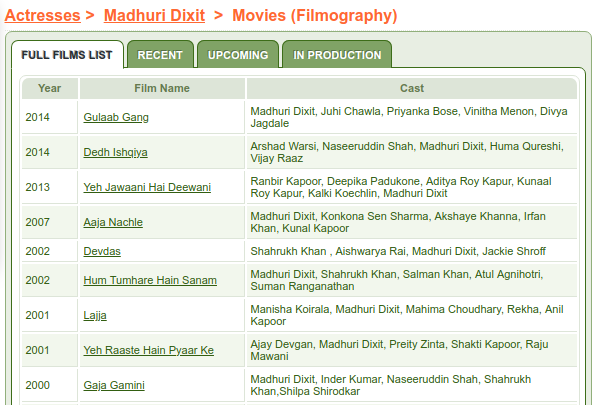
\includegraphics[scale=0.45]{figures/openweb/openweb-indian.png}
\caption[
The query \nl{list of Salman Khan and Madhuri Dixit movies}
requires compositional understanding.
]{The query \nl{list of Salman Khan and Madhuri Dixit movies}
requires filtering the list of entities
by the value in the Cast column.}
\label{fig:openweb-indian}
\end{figure}

\begin{figure}[tp]
\centering
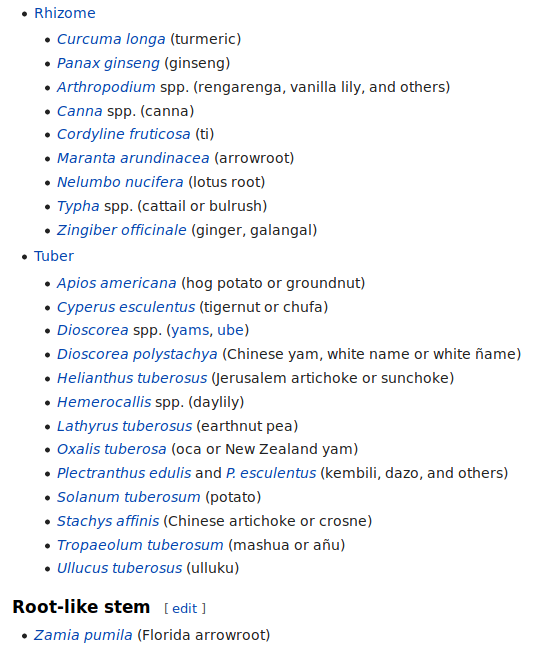
\includegraphics[scale=0.45]{figures/openweb/openweb-tubers.png}
\caption[
The query \nl{list of plants that are tubers}
requires compositional understanding.
]{The query \nl{list of plants that are tubers}
requires locating the correct portion of the list
based on the list indentation.}
\label{fig:openweb-tubers}
\end{figure}

%%%%%%%%%%

\begin{itemize}
\item In Figure~\ref{fig:openweb-hedgefund},
the query \nl{list of hedge funds in New York}
requires filtering the list of entities from
the Firm column by the values in the Headquarters column.
No extraction paths we defined can perform such filtering.

% \item In Figure~\ref{fig:openweb-ps3},
% the query \nl{list of PS3 games in 2012}
% similarly requires filtering for games
% where the Platforms column includes PS3 as one of the values.
% The results also have to be aggregated across four tables,
% one for each quarter.

\item In Figure~\ref{fig:openweb-indian},
the query \nl{list of Salman Khan and Madhuri Dixit movies}
requires finding movies that
have \emph{both} people in the Cast column.

\item In Figure~\ref{fig:openweb-tubers},
the query \nl{list of plants that are tubers}
requires identifying the correct subsection to extract
the entities from.
This requires understanding that list indentation
signifies membership to the category \emph{Tuber}.

\end{itemize}

We also observed that
data \emph{tables} on web pages provide a rich structure
suitable for compositional reasoning,
as illustrated in some of the examples above.
This observation serves as the inspiration
for the task of answering complex questions on web tables,
which we will cover in the subsequent chapters.

\section{Conclusion}

In this chapter,
we have explored the nature of semi-structured data
on web pages.
Instead of assuming a fixed data schema,
we use the DOM tree as a generic representation of the structures
on web pages.
The process of extracting HTML elements in the tree
is represented as an extraction path,
which is discrete and domain-independent.
To rank the extraction paths,
we use
structural and denotation features to
access the schematic information of the selected elements.
For instance, \Sc{Tag} structural features
help distinguish entities from non-entities
(e.g., \T{<a>} and \T{<td>} elements are more likely
to represent entities),
while \Sc{PhraseShape} denotation features
capture the types of the selected entities
(e.g., a phrase with the shape ``\T{Aa Aa}''
is likely to be a named entity).

Moving forward,
we are going to apply similar techniques
when we consider more complex questions
in the subsequent chapters.
The semi-structured knowledge source will be represented
using a generic graph representation
that can encode artibrary data schemata,
similar to the DOM tree representation used in this chapter.
The process of computing the answer
will be represented as \emph{logical forms},
which are discrete and domain-independent constructs 
like extraction paths,
but can also encode multi-step reasoning.
Features similar to structural and denotation features
presented here
will be used to rank the produced logical forms.
However, unlike the finite number of extraction paths,
it is rarely possible to enumerate all logical forms,
and thus we will extensively study
the methods to search over the space
of logical forms.
